\documentclass[twoside]{book}

% Packages required by doxygen
\usepackage{fixltx2e}
\usepackage{calc}
\usepackage{doxygen}
\usepackage[export]{adjustbox} % also loads graphicx
\usepackage{graphicx}
\usepackage[utf8]{inputenc}
\usepackage{makeidx}
\usepackage{multicol}
\usepackage{multirow}
\PassOptionsToPackage{warn}{textcomp}
\usepackage{textcomp}
\usepackage[nointegrals]{wasysym}
\usepackage[table]{xcolor}

% Font selection
\usepackage[T1]{fontenc}
\usepackage[scaled=.90]{helvet}
\usepackage{courier}
\usepackage{amssymb}
\usepackage{sectsty}
\renewcommand{\familydefault}{\sfdefault}
\allsectionsfont{%
  \fontseries{bc}\selectfont%
  \color{darkgray}%
}
\renewcommand{\DoxyLabelFont}{%
  \fontseries{bc}\selectfont%
  \color{darkgray}%
}
\newcommand{\+}{\discretionary{\mbox{\scriptsize$\hookleftarrow$}}{}{}}

% Page & text layout
\usepackage{geometry}
\geometry{%
  a4paper,%
  top=2.5cm,%
  bottom=2.5cm,%
  left=2.5cm,%
  right=2.5cm%
}
\tolerance=750
\hfuzz=15pt
\hbadness=750
\setlength{\emergencystretch}{15pt}
\setlength{\parindent}{0cm}
\setlength{\parskip}{3ex plus 2ex minus 2ex}
\makeatletter
\renewcommand{\paragraph}{%
  \@startsection{paragraph}{4}{0ex}{-1.0ex}{1.0ex}{%
    \normalfont\normalsize\bfseries\SS@parafont%
  }%
}
\renewcommand{\subparagraph}{%
  \@startsection{subparagraph}{5}{0ex}{-1.0ex}{1.0ex}{%
    \normalfont\normalsize\bfseries\SS@subparafont%
  }%
}
\makeatother

% Headers & footers
\usepackage{fancyhdr}
\pagestyle{fancyplain}
\fancyhead[LE]{\fancyplain{}{\bfseries\thepage}}
\fancyhead[CE]{\fancyplain{}{}}
\fancyhead[RE]{\fancyplain{}{\bfseries\leftmark}}
\fancyhead[LO]{\fancyplain{}{\bfseries\rightmark}}
\fancyhead[CO]{\fancyplain{}{}}
\fancyhead[RO]{\fancyplain{}{\bfseries\thepage}}
\fancyfoot[LE]{\fancyplain{}{}}
\fancyfoot[CE]{\fancyplain{}{}}
\fancyfoot[RE]{\fancyplain{}{\bfseries\scriptsize Generated by Doxygen }}
\fancyfoot[LO]{\fancyplain{}{\bfseries\scriptsize Generated by Doxygen }}
\fancyfoot[CO]{\fancyplain{}{}}
\fancyfoot[RO]{\fancyplain{}{}}
\renewcommand{\footrulewidth}{0.4pt}
\renewcommand{\chaptermark}[1]{%
  \markboth{#1}{}%
}
\renewcommand{\sectionmark}[1]{%
  \markright{\thesection\ #1}%
}

% Indices & bibliography
\usepackage{natbib}
\usepackage[titles]{tocloft}
\setcounter{tocdepth}{3}
\setcounter{secnumdepth}{5}
\makeindex

% Hyperlinks (required, but should be loaded last)
\usepackage{ifpdf}
\ifpdf
  \usepackage[pdftex,pagebackref=true]{hyperref}
\else
  \usepackage[ps2pdf,pagebackref=true]{hyperref}
\fi
\hypersetup{%
  colorlinks=true,%
  linkcolor=blue,%
  citecolor=blue,%
  unicode%
}

% Custom commands
\newcommand{\clearemptydoublepage}{%
  \newpage{\pagestyle{empty}\cleardoublepage}%
}

\usepackage{caption}
\captionsetup{labelsep=space,justification=centering,font={bf},singlelinecheck=off,skip=4pt,position=top}

%===== C O N T E N T S =====

\begin{document}

% Titlepage & ToC
\hypersetup{pageanchor=false,
             bookmarksnumbered=true,
             pdfencoding=unicode
            }
\pagenumbering{alph}
\begin{titlepage}
\vspace*{7cm}
\begin{center}%
{\Large Test Project \\[1ex]\large v0.\+0 }\\
\vspace*{1cm}
{\large Generated by Doxygen 1.8.13}\\
\end{center}
\end{titlepage}
\clearemptydoublepage
\pagenumbering{roman}
\tableofcontents
\clearemptydoublepage
\pagenumbering{arabic}
\hypersetup{pageanchor=true}

%--- Begin generated contents ---
\chapter{Class Index}
\section{Class List}
Here are the classes, structs, unions and interfaces with brief descriptions\+:\begin{DoxyCompactList}
\item\contentsline{section}{\hyperlink{classStopWatch}{Stop\+Watch} }{\pageref{classStopWatch}}{}
\item\contentsline{section}{\hyperlink{structValue}{Value} }{\pageref{structValue}}{}
\end{DoxyCompactList}

\chapter{Class Documentation}
\hypertarget{classStopWatch}{}\section{Stop\+Watch Class Reference}
\label{classStopWatch}\index{Stop\+Watch@{Stop\+Watch}}
\subsection*{Public Member Functions}
\begin{DoxyCompactItemize}
\item 
\mbox{\Hypertarget{classStopWatch_a4d11f9e0d4c77c8df78313e9e0643fca}\label{classStopWatch_a4d11f9e0d4c77c8df78313e9e0643fca}} 
void {\bfseries start\+Clock} ()
\item 
\mbox{\Hypertarget{classStopWatch_a2bf9c1940bc13449bace7be4626d78ec}\label{classStopWatch_a2bf9c1940bc13449bace7be4626d78ec}} 
void {\bfseries capture\+Finish\+Time} ()
\item 
\mbox{\Hypertarget{classStopWatch_afe6f7fc75f5ce4f2901383e1f6e020e8}\label{classStopWatch_afe6f7fc75f5ce4f2901383e1f6e020e8}} 
double {\bfseries report\+Finish\+Time} ()
\item 
\mbox{\Hypertarget{classStopWatch_ae49d0704410ca4e30be49ba9e471bc3f}\label{classStopWatch_ae49d0704410ca4e30be49ba9e471bc3f}} 
void {\bfseries report\+Raw\+Times} ()
\end{DoxyCompactItemize}


The documentation for this class was generated from the following files\+:\begin{DoxyCompactItemize}
\item 
Stop\+Watch.\+hpp\item 
Stop\+Watch.\+cpp\end{DoxyCompactItemize}

\hypertarget{structValue}{}\section{Value Struct Reference}
\label{structValue}\index{Value@{Value}}


Collaboration diagram for Value\+:\nopagebreak
\begin{figure}[H]
\begin{center}
\leavevmode
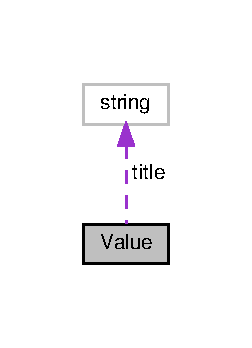
\includegraphics[width=121pt]{structValue__coll__graph}
\end{center}
\end{figure}
\subsection*{Public Member Functions}
\begin{DoxyCompactItemize}
\item 
\mbox{\Hypertarget{structValue_ab62780d112b99503bb67b5b4220a54b8}\label{structValue_ab62780d112b99503bb67b5b4220a54b8}} 
{\bfseries Value} (string \&filename)
\item 
\mbox{\Hypertarget{structValue_a12f446c1de93ebcffa83b792434a6d45}\label{structValue_a12f446c1de93ebcffa83b792434a6d45}} 
void {\bfseries set\+Title} (string \&filename)
\item 
\mbox{\Hypertarget{structValue_abcfa5f07be1a11fc23cb77ed38361c60}\label{structValue_abcfa5f07be1a11fc23cb77ed38361c60}} 
unsigned int {\bfseries count\+Words} (string const \&str)
\item 
\mbox{\Hypertarget{structValue_a9750bd014214587c5adeb7af03c3e844}\label{structValue_a9750bd014214587c5adeb7af03c3e844}} 
void {\bfseries set\+Count} (string \&filename)
\item 
\mbox{\Hypertarget{structValue_a9a07ab329fd770cda9a615dfa3387ebf}\label{structValue_a9a07ab329fd770cda9a615dfa3387ebf}} 
void {\bfseries report\+Value} ()
\end{DoxyCompactItemize}
\subsection*{Public Attributes}
\begin{DoxyCompactItemize}
\item 
\mbox{\Hypertarget{structValue_aae3d3accff785db290710b8475251775}\label{structValue_aae3d3accff785db290710b8475251775}} 
string {\bfseries title} = \char`\"{}\char`\"{}
\item 
\mbox{\Hypertarget{structValue_afcdc88ae3a5935947696704150e154fd}\label{structValue_afcdc88ae3a5935947696704150e154fd}} 
int {\bfseries line\+\_\+count} = 0
\item 
\mbox{\Hypertarget{structValue_a84f78f7074a5bbefcc5133e60edb6685}\label{structValue_a84f78f7074a5bbefcc5133e60edb6685}} 
int {\bfseries par\+\_\+count} = 0
\item 
\mbox{\Hypertarget{structValue_ae519294be41eb730d31d0b4123dee2ab}\label{structValue_ae519294be41eb730d31d0b4123dee2ab}} 
int {\bfseries word\+\_\+count} = 0
\item 
\mbox{\Hypertarget{structValue_ac353afa54a9674eb24f7d028ea6b7287}\label{structValue_ac353afa54a9674eb24f7d028ea6b7287}} 
int {\bfseries char\+\_\+count} = 0
\end{DoxyCompactItemize}
\subsection*{Static Public Attributes}
\begin{DoxyCompactItemize}
\item 
\mbox{\Hypertarget{structValue_a6c4e7b71cbac186ef94edf7fc81fbe6e}\label{structValue_a6c4e7b71cbac186ef94edf7fc81fbe6e}} 
static int {\bfseries total\+\_\+change\+\_\+count} = 0
\end{DoxyCompactItemize}


The documentation for this struct was generated from the following files\+:\begin{DoxyCompactItemize}
\item 
Value.\+hpp\item 
Value.\+cpp\end{DoxyCompactItemize}

%--- End generated contents ---

% Index
\backmatter
\newpage
\phantomsection
\clearemptydoublepage
\addcontentsline{toc}{chapter}{Index}
\printindex

\end{document}
